\documentclass{beamer}

\usetheme{Madrid}
\usecolortheme{rose}

\title{Projekt: Cloud Programming}
\subtitle{Phase 2}
\author{Jonas Habel}
\date{\today}

\usepackage{tabularx}
\usepackage{ragged2e}

\begin{document}

\begin{frame}
  \titlepage
\end{frame}

\begin{frame}{Agenda}
  \tableofcontents
\end{frame}

\section{Aufgabenstellung}
\begin{frame}{Aufgabenstellung}
  \begin{itemize}
    \item Einrichten der Cloud Architektur der Unternehmenswebsite
    \item Website muss hochverfügbar sein
    \item Nutzende aus der ganzen Welt sollen keine Verzögerung erfahren
    \item Automatisches skalieren wenn es viele Anfragen gibt.
  \end{itemize}
\end{frame}

\section{Vorgehensweise}
\begin{frame}{Vorgehensweise}
\begin{figure}[h]
\centering
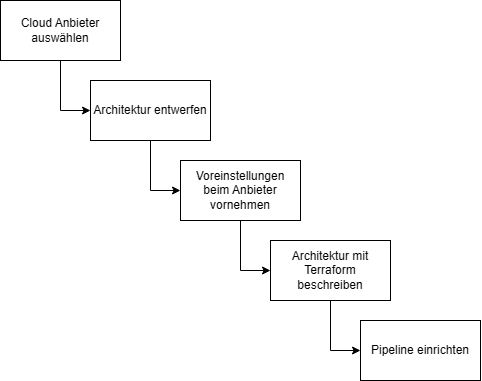
\includegraphics[width=.8\textwidth]{pics/Vorgehensweise.png}
\end{figure}
\end{frame}


\section{Cloud Anbieter auswählen}
\begin{frame}{AWS vs. Azure: Kosten \& Anforderungen}
\small
\renewcommand{\arraystretch}{1.2}

\begin{tabular}{p{0.17\textwidth}p{0.35\textwidth}p{0.35\textwidth}}
\hline
\textbf{Anforderung} & \textbf{AWS} & \textbf{Azure} \\
\hline
Hochverfügbare Website &
Multi-AZ + Load Balancer &
Container Apps in 2 Regionen + Front Door (Failover/Load-Balancing) \\
\hline
Weltweit ohne Verzögerung &
CloudFront (CDN) + global DNS &
Front Door + optional CDN/Caching \\
\hline
Auto-Scaling bei Last &
Auto Scaling / ECS/EKS / Lambda &
Container Apps Autoscaling + Front Door \\
\hline
Kosten &
ähnlich; Treiber: Compute + Egress + Multi-AZ/Region &
ähnlich; Treiber: Container Apps + Egress + Front Door + 2 Regionen \\
\hline
\end{tabular}

\vspace{0.4em}
\begin{block}{Auswahl}
Die Auswahl ist auf Azure gefallen, da die Kosten vergleichbar sind und dieses bereits im Unternehmen Verwendung findet.
\end{block}
\end{frame}

\section{Architekturentwurf}
\begin{frame}{Architekturentwurf}
\begin{figure}[h]
\centering
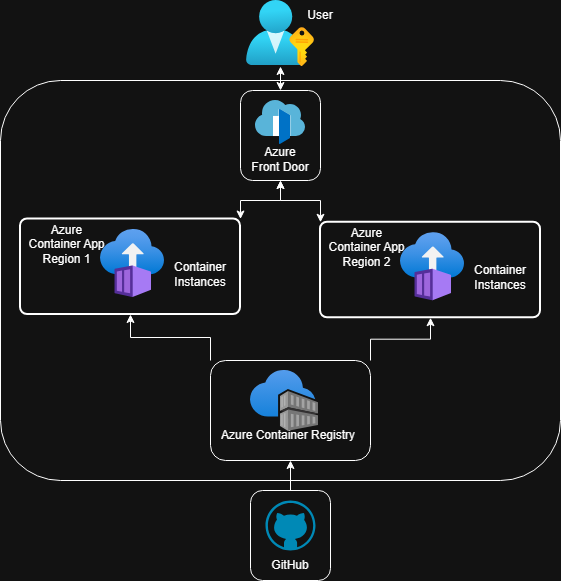
\includegraphics[width=.64\textwidth]{pics/CloudArchitecture.Compact.png}
\end{figure}
\end{frame}

\section{Voreinstellungen}
\begin{frame}{Voreinstellungen}
\begin{itemize}
  \item Azure CLI installiert
  \item Terraform installiert
  \item Docker installiert
  \item Azure subscription
  \item App registration in Azure (Mircrosoft Entra ID $\rightarrow$ App registrations)
  \item Client Secret für die registrierte App für CLI Zugriff
\end{itemize}
\end{frame}

\begin{frame}[fragile]{Script ausführen}
  Mit Hilfe des \texttt{terroform-local.cmd} Skripts kann der gesamte Bereitstellungsprozess lokal ausgeführt werden. Dazu müssen die folgenden Umgebungsvariables gesetzt werden:
  \begin{itemize}
    \item \texttt{ACR\_NAME, ACR\_RESOURCE\_GROUP, ACR\_LOCATION}
    \item \texttt{APP\_ID}
    \item \texttt{TENANT\_ID}
    \item \texttt{CLIENT\_SECRET}
    \item \texttt{IMAGE\_NAME, IMAGE\_TAG}
    \item \texttt{TFSTATE\_RESOURCE\_GROUP, TF\_STATE\_STORAGE\_ACCOUNT, TF\_STATE\_CONTAINER, TFSTATE\_KEY}
  \end{itemize}
\end{frame}
\begin{frame}{Skript ausführen}
  Zum Ausführen muss der folgende Befehl vom Root Verzeichnis des Projekts in einer Kommandozeile eigegeben werden:
  \begin{block}{Command}
    \texttt{scripts\textbackslash terraform-local.cmd}
  \end{block}
  Das Skript durchläuft die folgenden Schritte:
  \begin{itemize}
    \item Login in Azure mit Service Principal.
    \item (optional) Docker-Image bauen und nach ACR pushen.
    \item Terraform mit Remote-Backend initialisieren.
    \item Terraform anwenden, um Infrastruktur zu erstellen/aktualisieren.
  \end{itemize}
\end{frame}

\section{Anforderungen und Umsetzung}
\begin{frame}{Anforderungen und Umsetzung}
  \begin{itemize}
    \item Hochverfügbarkeit: Zwei regionale Container Apps (primary/secondary) hinter Front Door
    \begin{block}{Azure Front Door}
       https://learn.microsoft.com/de-de/azure/frontdoor/front-door-overview
    \end{block}
    \item Weltweite Besucher: Front Door als globaler Einstiegspunkt mit Geo-Routing und Anycast.
    \item Autoscaling: Container Apps skalieren automatisch nach HTTP-Last (min/max Replikas)  
     \begin{block}{Azure Container Apps}
https://learn.microsoft.com/en-us/azure/container-apps/overview

  \end{block}
  \end{itemize}
\end{frame}

\section{Pipeline in GitHub}
\begin{frame}{Pipeline in GitHub}
\begin{figure}[h]
\centering
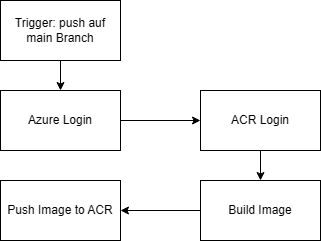
\includegraphics[width=.8\textwidth]{pics/PipelineAblauf.png}
\end{figure}
\end{frame}

\section{Das erfolgreiche Deployment}
\begin{frame}{Das erfolgreiche Deployment}
\begin{figure}[h]
\centering
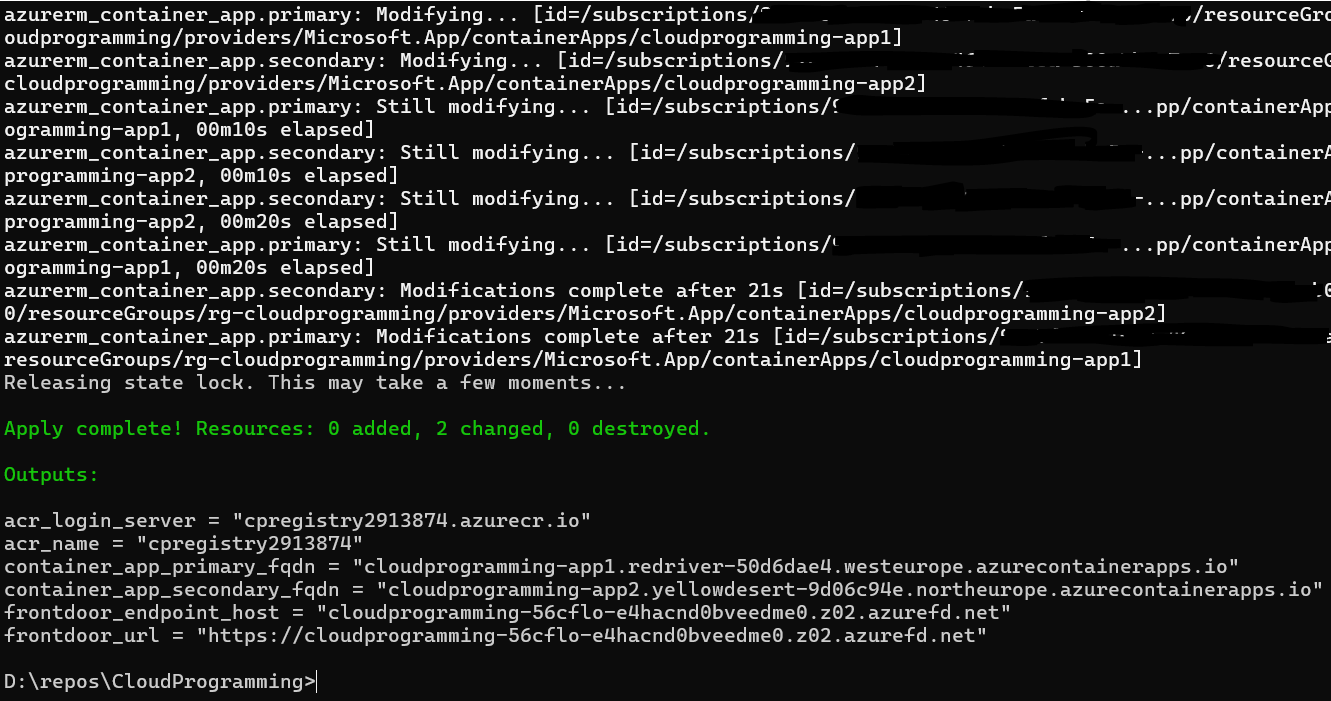
\includegraphics[width=1\textwidth]{pics/cmd.png}
\end{figure}
\end{frame}

\begin{frame}{Das erfolgreiche Deployment}
\begin{figure}[h]
\centering
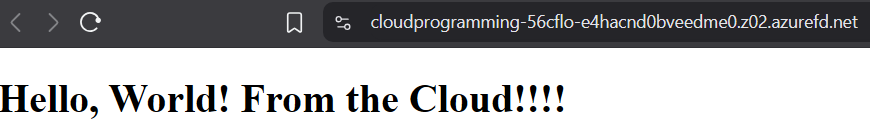
\includegraphics[width=1\textwidth]{pics/browser.png}
\end{figure}
\end{frame}

\end{document}
